Let's now recall for a moment the Hodgkin-Huxley model:
\begin{equation*}
    C\frac{dV}{dt}=-\bar{g}_{Na}m^{3}h(V-E_{Na})-\bar{g}_{K}n^{4}(V-E_{K})-g_{leak}(V-E_{leak})+I_{app}
\end{equation*}
The dynamics of the gating particles is reported here and depicted below:
\begin{align*}
    \frac{dm}{dt} & =\alpha_{m}(V)(1-m)-\beta_{m}(V)m \\
    \frac{dh}{dt} & =\alpha_{h}(V)(1-h)-\beta_{h}(V)h \\
    \frac{dn}{dt} & =\alpha_{n}(V)(1-n)-\beta_{n}(V)n
\end{align*}
\begin{figure}[H]
    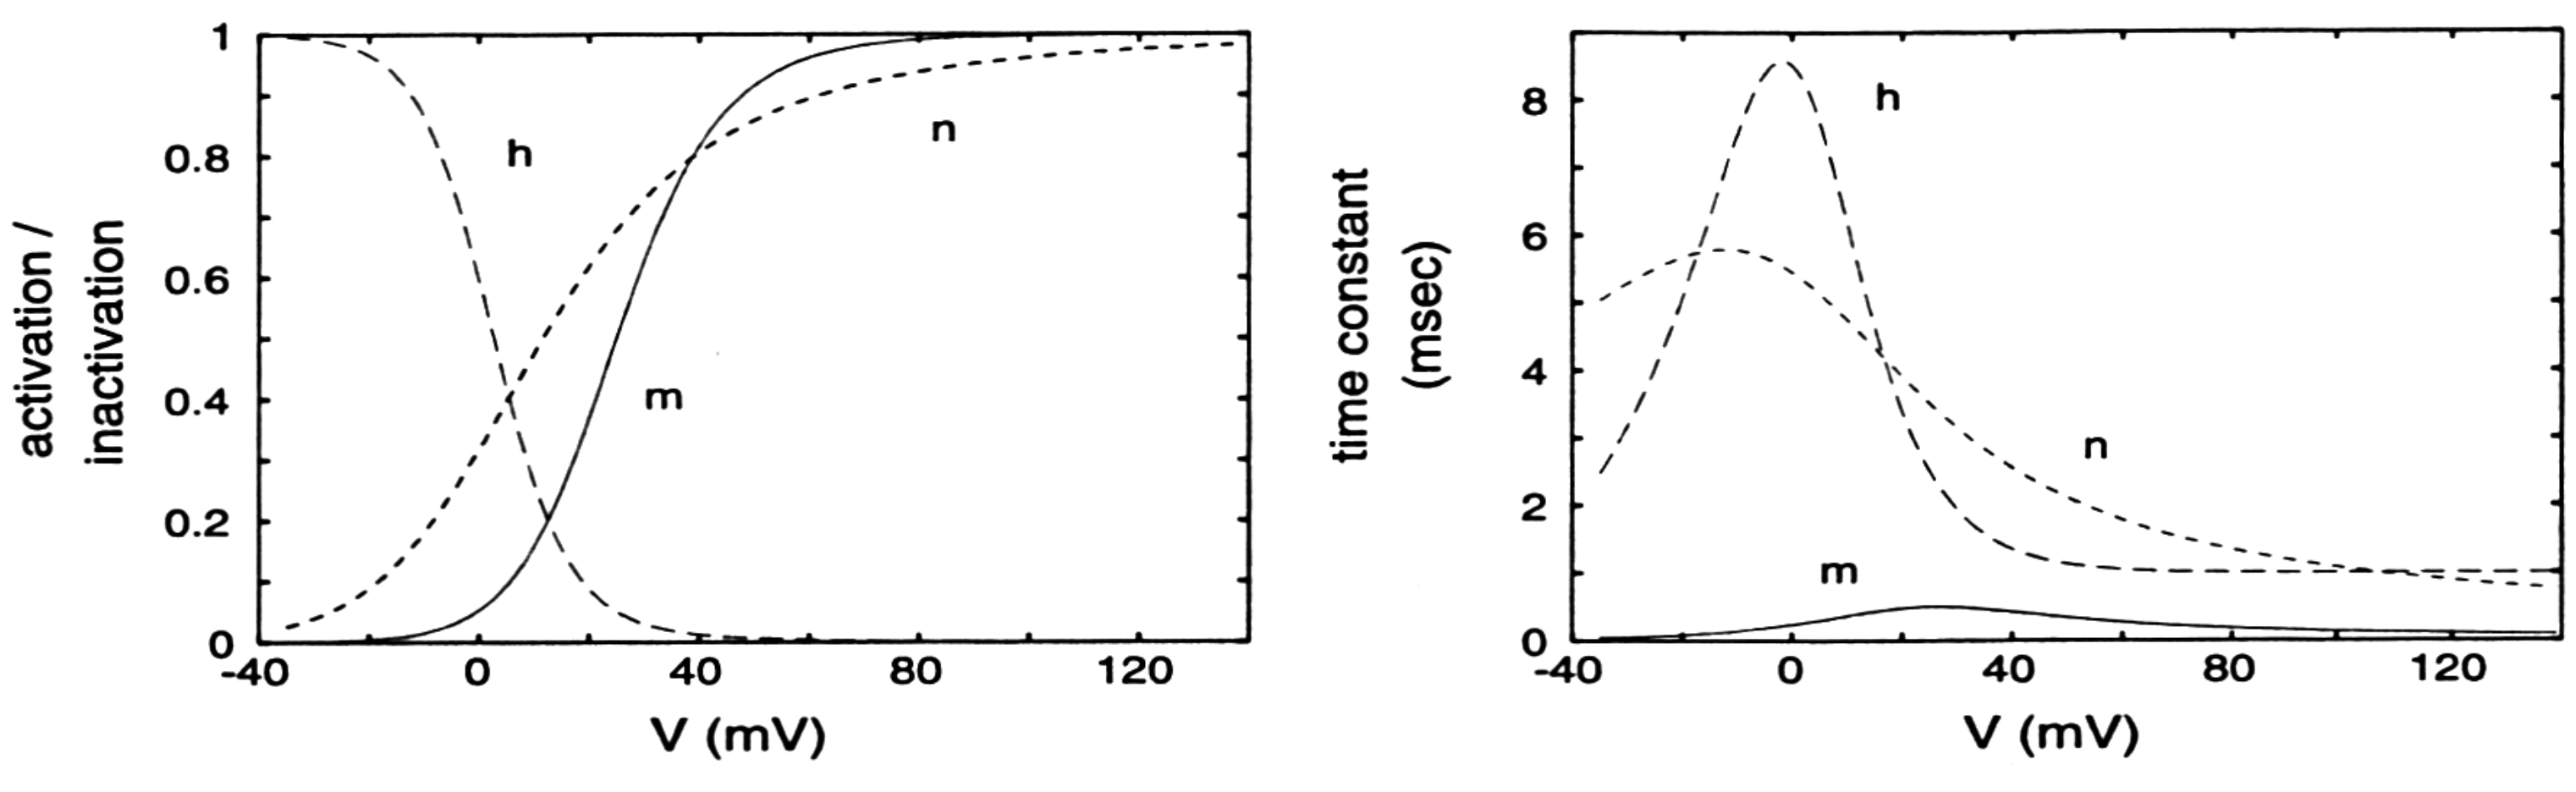
\includegraphics[scale=0.25]{09_1}
    \centering
\end{figure}
The goal now is to switch from a model described by four differential equations (as the HH one), to
a model with reduced complexity, described only by two equations. Henceforth, some simplifications
are to be done:
\begin{enumerate}
    \item The \(\tau_{m}\) time constant, related to the gating particle \(m\), is extremely small if
          compared to \(\tau_{h}\) and \(\tau_{n}\), implying an almost instantaneous depolarization. Therefore,
          it can be said that the action potential peak due to \(m\) occurs immediately and that \(m\) presents
          no transient behaviour, assuming immediately its steady-state value (quasi-steady state approximation):
          \begin{equation*}
              m(t)\to{m_{\infty}\Bigl(V(t)\Bigr)}
          \end{equation*}
    \item By looking at the time constants \(\tau_{h}\) and \(\tau_{n}\), they are similar in magnitude,
          therefore the activation/inactivation of \(h\) and \(n\) gating particles occurs with a similar
          temporal dynamics. The two gating particles present a sort of oppsite sigmoidal behaviour, thus
          it can be said that at steady state the following relationship holds:
          \begin{equation*}
              n_{\infty}(V)\approx{1-h_{\infty}(V)}
          \end{equation*}
\end{enumerate}
Now, since it has been shown that \(n\) and \((1-h)\) present similar kinetics, they can be substituted by
a new variable \(w\), in particular \(w=b-h=a\cdot{n}\) with \(a=b=1\) in the considered case, leading to:
\begin{equation*}
    w=1-h=n
\end{equation*}
Henceforth, the HH state equation can be rewritten as follow:
\begin{gather*}
    C\frac{dV}{dt}=-\bar{g}_{Na}m^{3}h(V-E_{Na})-\bar{g}_{K}n^{4}(V-E_{K})-g_{leak}(V-E_{leak})+I_{app}\\
    \downarrow\\
    C\frac{dV}{dt}=-\bar{g}_{Na}m_{\infty}(b-w)(V-E_{Na})-\bar{g}_{K}\Bigl(\frac{w}{a}\Bigr)^{4}(V-E_{K})-g_{leak}(V-E_{leak})+I_{app}
\end{gather*}
The two gating particles present the following dynamics:
\begin{align*}
    \frac{dm}{dt} & =0\Rightarrow{\text{no transient is considered for \(m\), only its steady-state value}} \\
    \frac{dw}{dt} & =\frac{1}{\tau_{w}}G(V,w)
\end{align*}
Note that the function \(G(V,w)\) is an extra degree of freedom which allows to derived different neuron models.

\subsection{The Morris-Lecar Model}
In this model sodium channels are disregarded, while the calcium ones are taken into account, together with the
potassium channels. Here the gating particle \(w\) is substituted by \(N\), but the meaning is the same.
The model obtained is described by the two following equations:
\begin{gather*}
    C\frac{dV}{dt}=-g_{Ca}M_{SS}(V-E_{Ca})-g_{K}N(V-E_{K})-g_{leak}(V-E_{leak})+I_{app}\\
    \frac{dN}{dt}=\frac{N-N_{SS}}{\tau_{N}}
\end{gather*}
The Morris-Lecar model is capable of simulating several distinct patterns of activity.
\begin{figure}[H]
    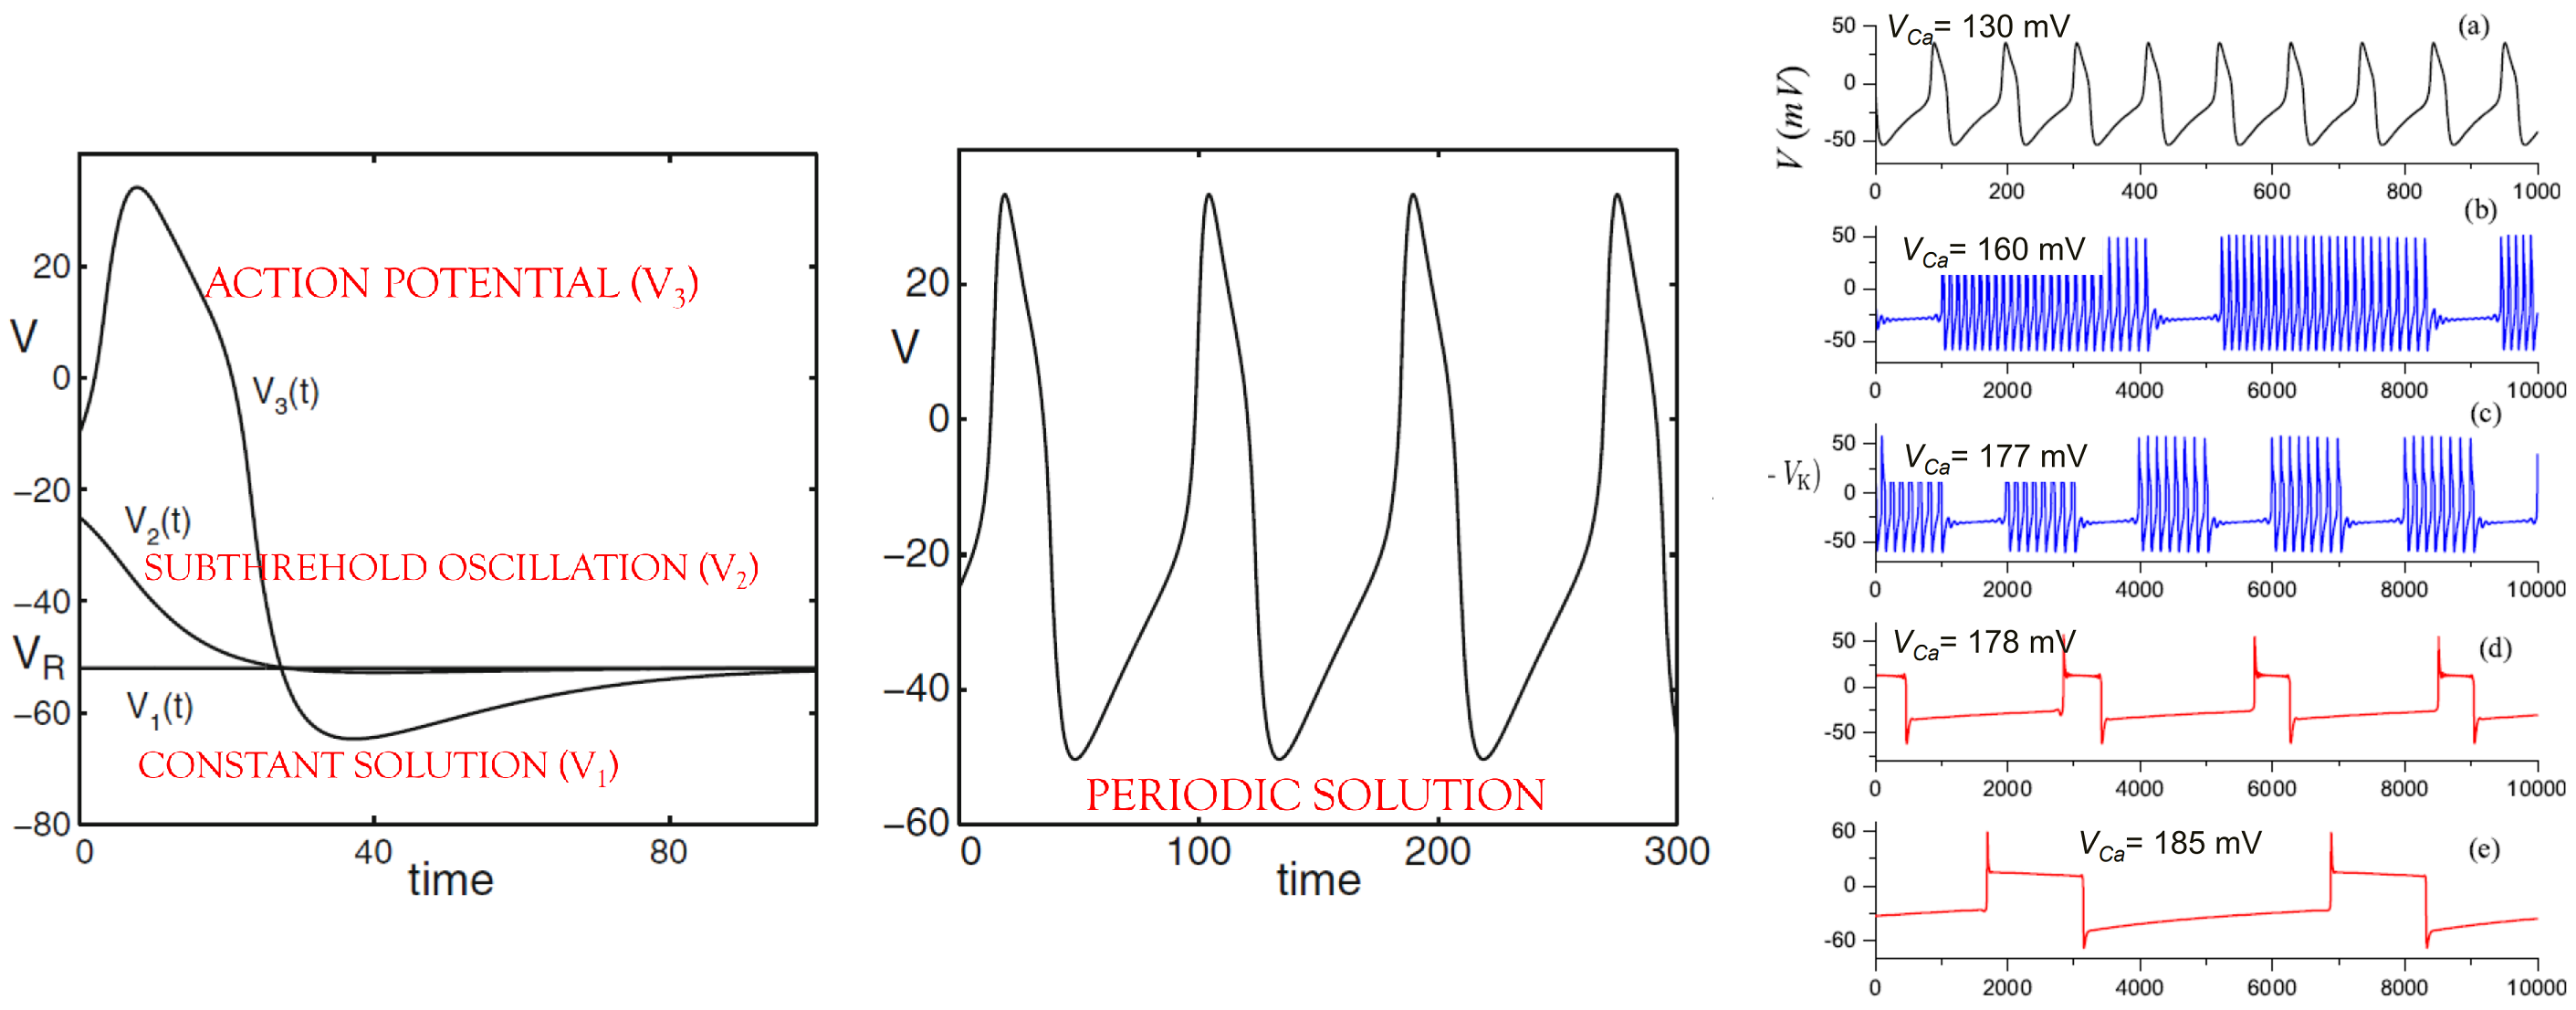
\includegraphics[scale=0.275]{09_2}
    \centering
\end{figure}
The two differential equations describing the model can be rewritten in a generic form:
\begin{equation*}
    \frac{dV}{dt}=f(V,N)\hspace{2.5cm}\text{and}\hspace{2.5cm}\frac{dN}{dt}=G(V,N)
\end{equation*}
Given a generic solution of the system in the \(\Bigl(V(t),N(t)\Bigr)\) form, each instant \(t^{*}\) defines
a point in the phase plane. By changing \(t^{*}\) and collecting several points, trajectories and
orbits are obtained. Let's now set some definitions:
\begin{itemize}
    \item \textbf{Fixed Point}: it is an equilibrium point \(R\), such that \(f(V_{R},N_{R})=G(V_{R},N_{R})=0\),
          leading to a \textit{constant solution}.
    \item \textbf{Closed Orbit}: this implies a \textit{periodic solution}.
    \item \textbf{Nullcline}: trajectories where \(\frac{dV}{dt}=f(V,N)=0\) (\(V\)-nullcline) or
          \(\frac{dN}{dt}=G(V,N)=0\) (\(N\)-nullcline).
\end{itemize}
Note that nullclines intersect at fixed points, which can be either stable or unstable.
\begin{figure}[H]
    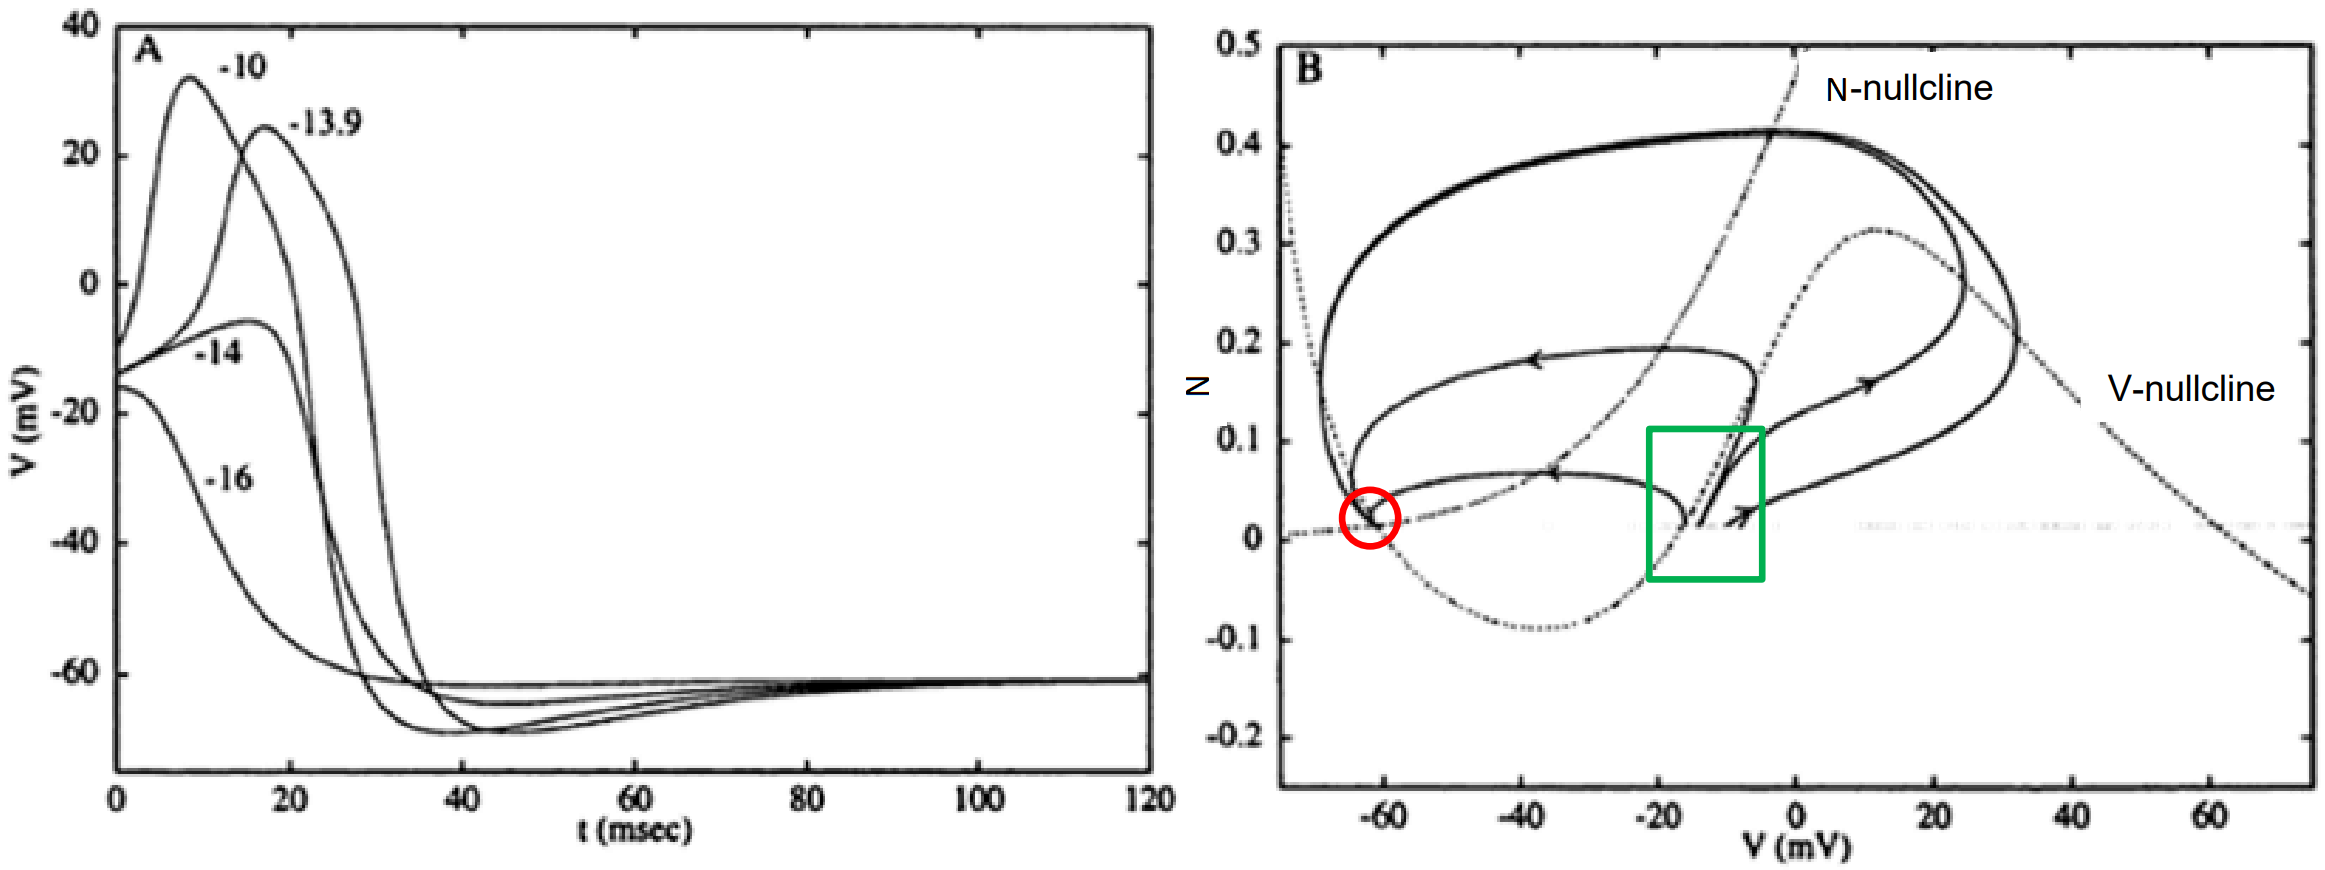
\includegraphics[scale=0.3]{09_3}
    \centering
\end{figure}
Each trajectory of the ones showed above has different initial points, according to the stimulation current
\(I_{app}\), however all of them tends to the same point \(P\), which is thus a global attractor,
in particular \(V_{P}=E_{rest}\) and \(N_{P}=N_{\infty}\). Note that the global attractor is itself a
fixed point and it is located at the intersection of nullclines.\\
A periodic solution corresponds to a closed curve, thus an orbit. There is a unique fixed point, which
is unstable. On the contrary, in case of bistable models, there are both a stable fixed point and a
stable periodic orbit.
\begin{figure}[H]
    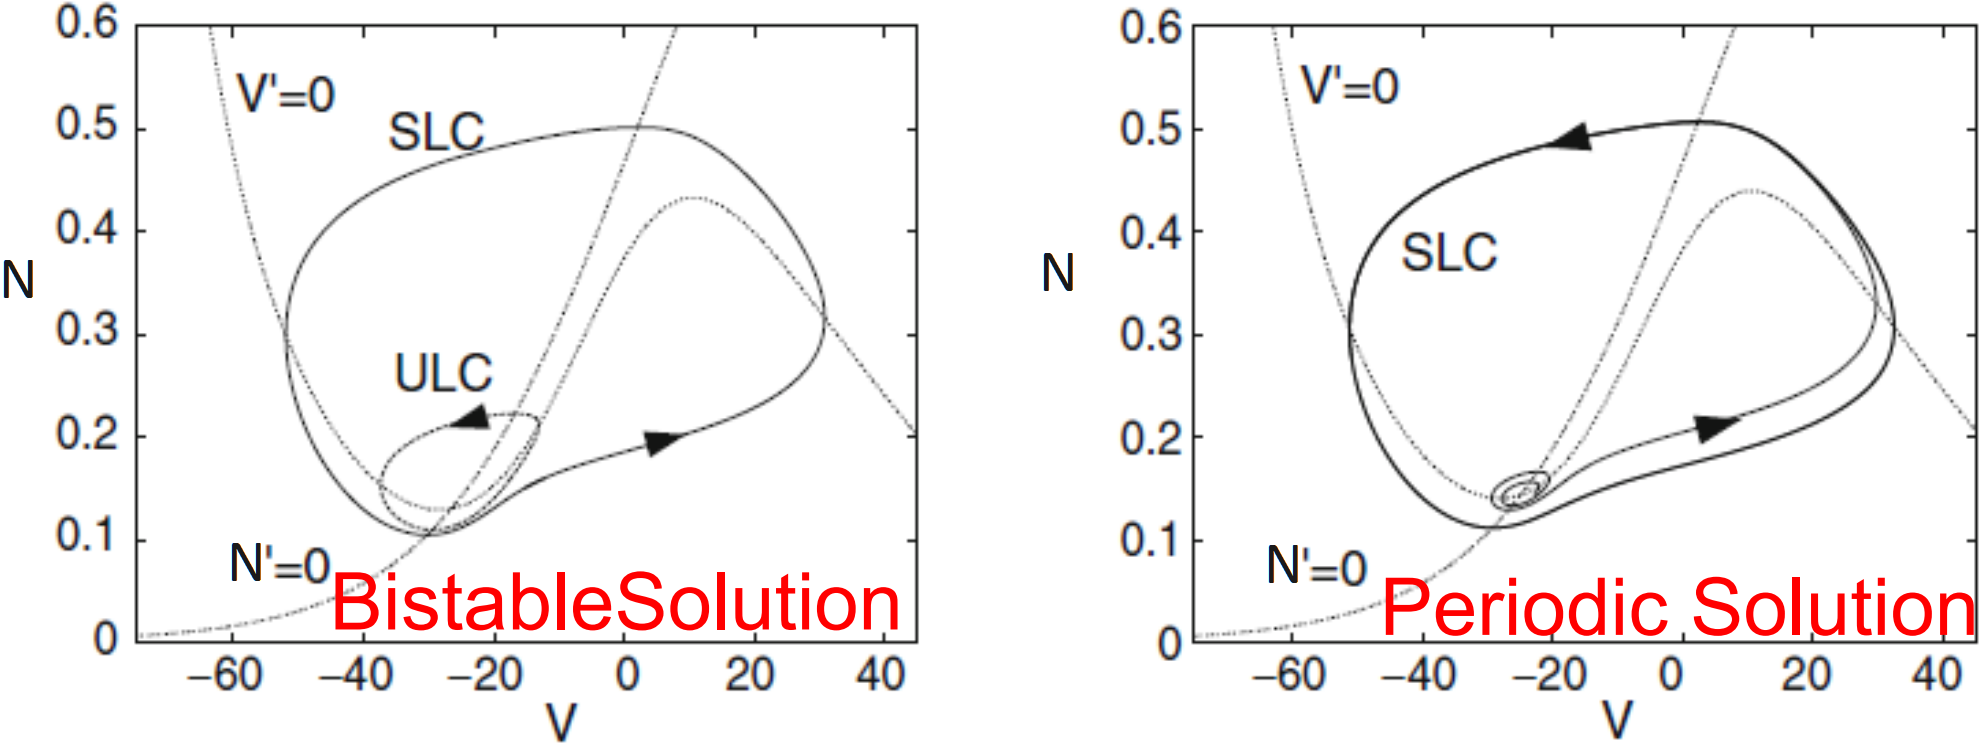
\includegraphics[scale=0.33]{09_4}
    \centering
\end{figure}

\subsection{The Fitzhugh-Nagumo Model}
This is the simplest 2D - i.e., described by two differential equations - model. The goal is to learn the
current that should be supplied to the system in order to elicit a certain type of activity. This model
does not provide a clear biophysical meaning, the equivalent circuit is no longer a reproduction of
the natural structures present in a neuron. It consists of:
\begin{itemize}
    \item A voltage-like variable \(u\) with a cubic non-linearity, allowing a regenerative self-excitation
          via a positive feedback.
    \item A recovery variable \(w\) having a linear dynamics, providing a slower negative feedback.
\end{itemize}
The model is thus described by:
\begin{equation*}
    \frac{du}{dt}=u-\frac{u^{3}}{3}-w+I_{app}
    \hspace{2.5cm}
    \text{and}
    \hspace{2.5cm}
    \frac{dw}{dt}=\epsilon{u+\beta-\gamma{W}}
\end{equation*}
with \(\beta\), \(\gamma\) and \(\epsilon\) being constants.
\begin{figure}[H]
    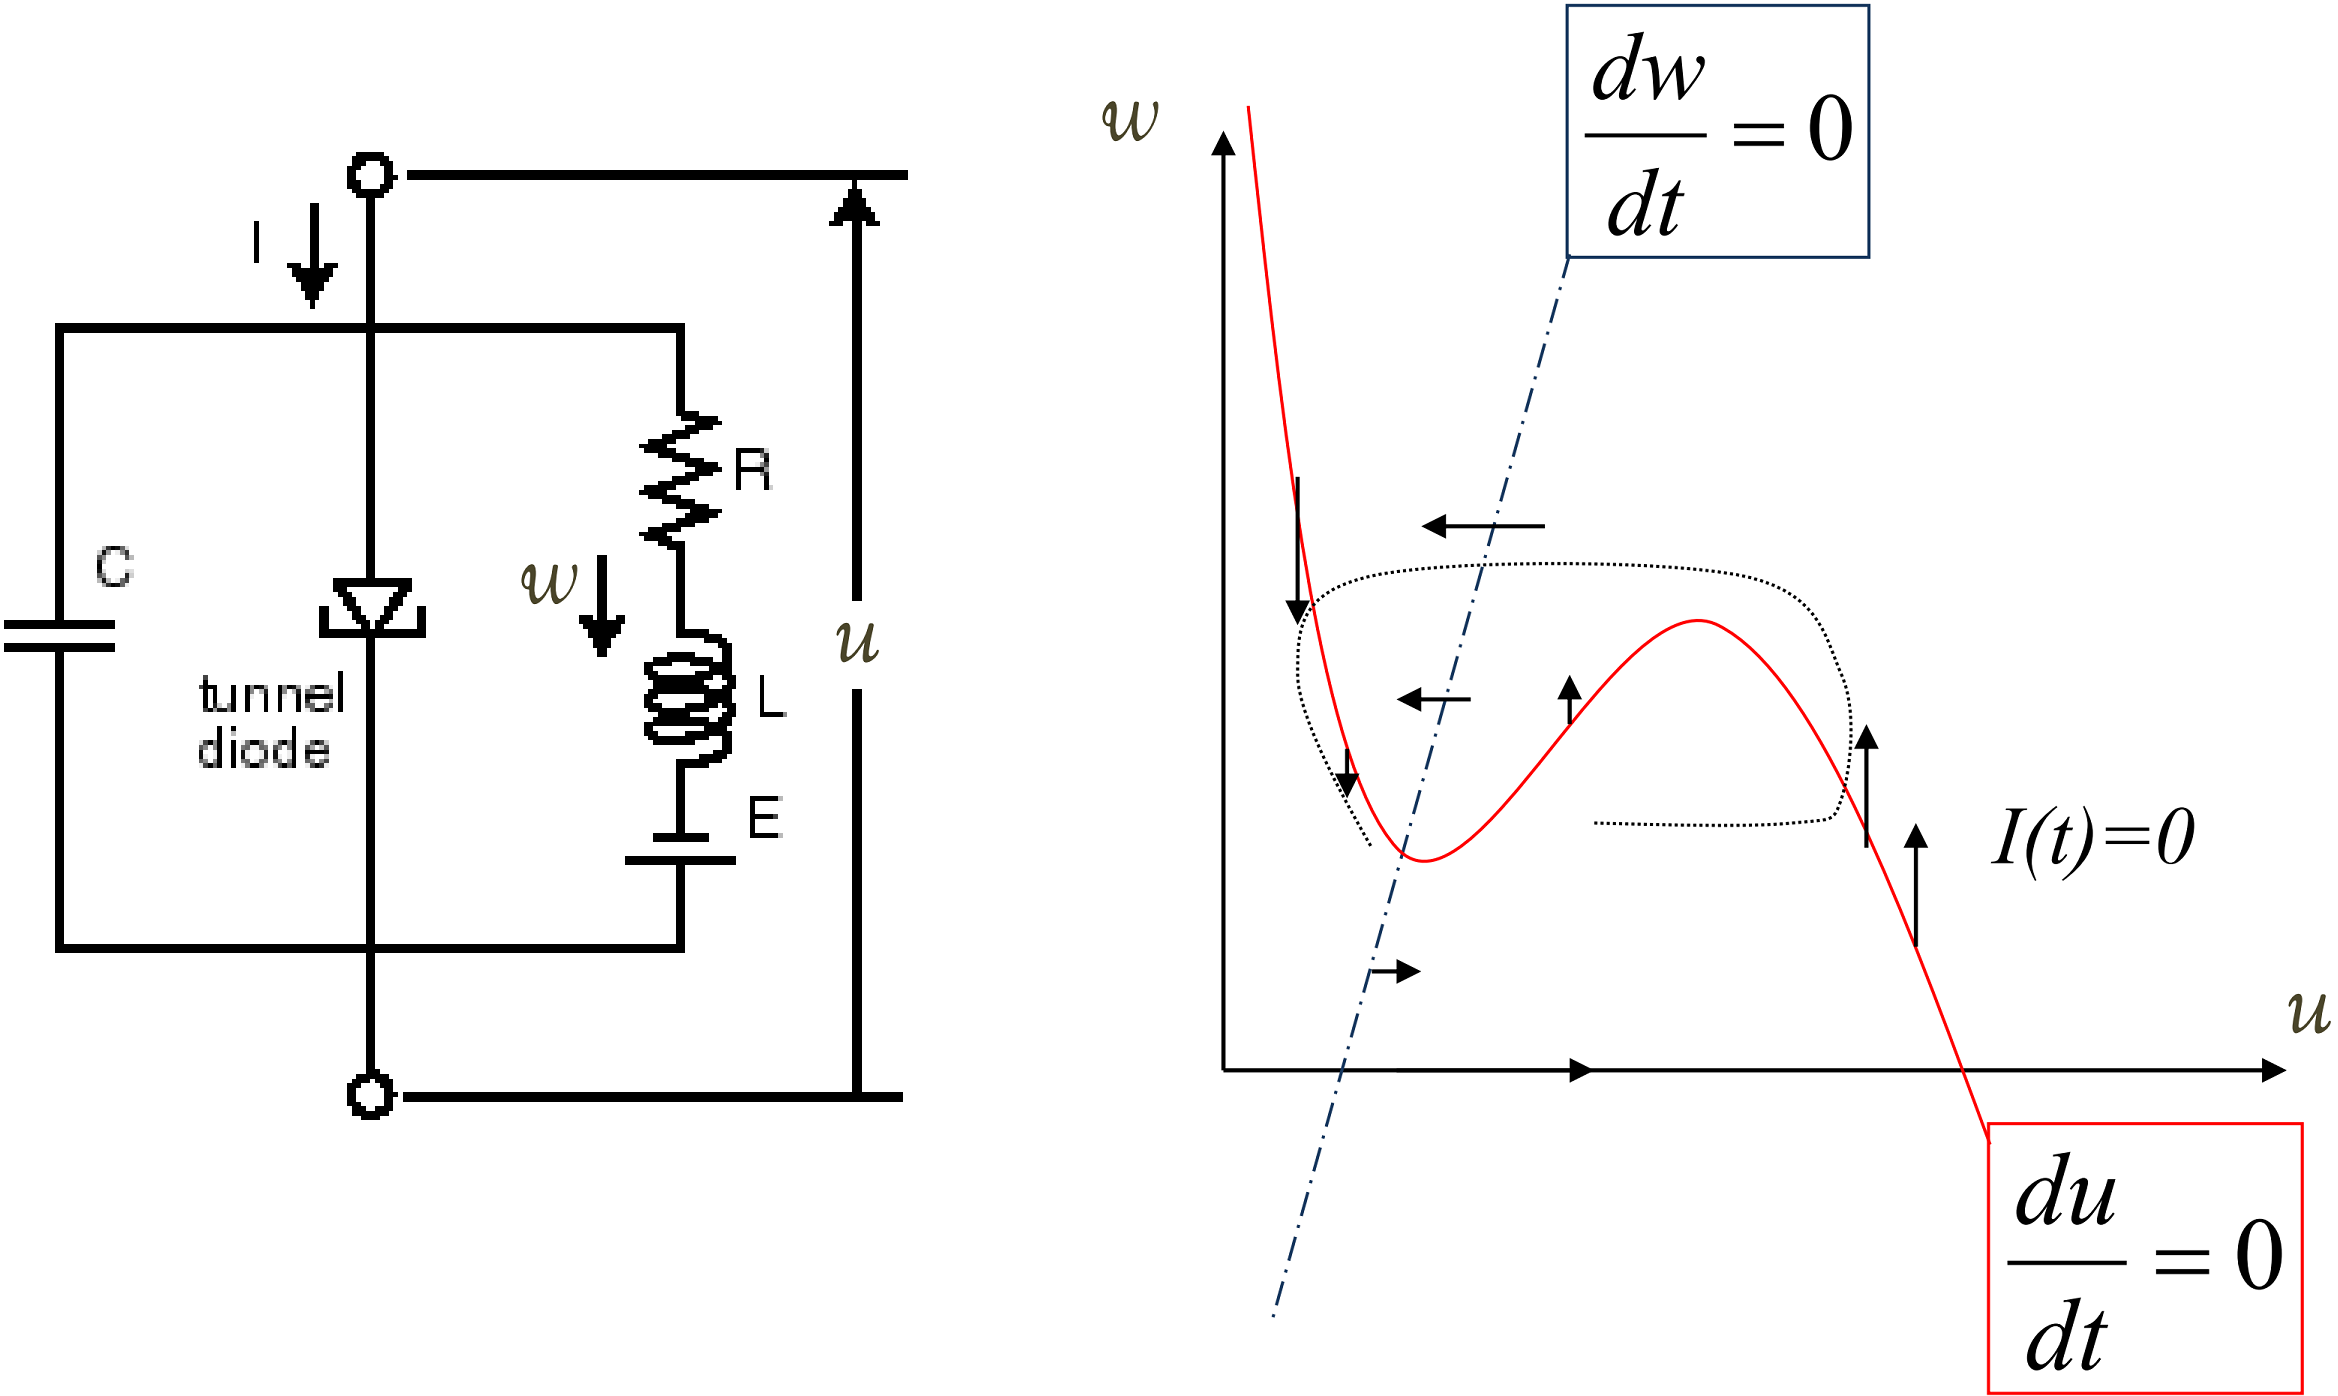
\includegraphics[scale=0.2]{09_5}
    \centering
\end{figure}
Note that for \(I(t)=0\) there is convergence toward a stable fixed point, otherwise an unstable
fixed point is obtained, leading to an orbit.\\
In general, the state of the model can be determined by looking at the trajectories on the phase plane.
\begin{figure}[H]
    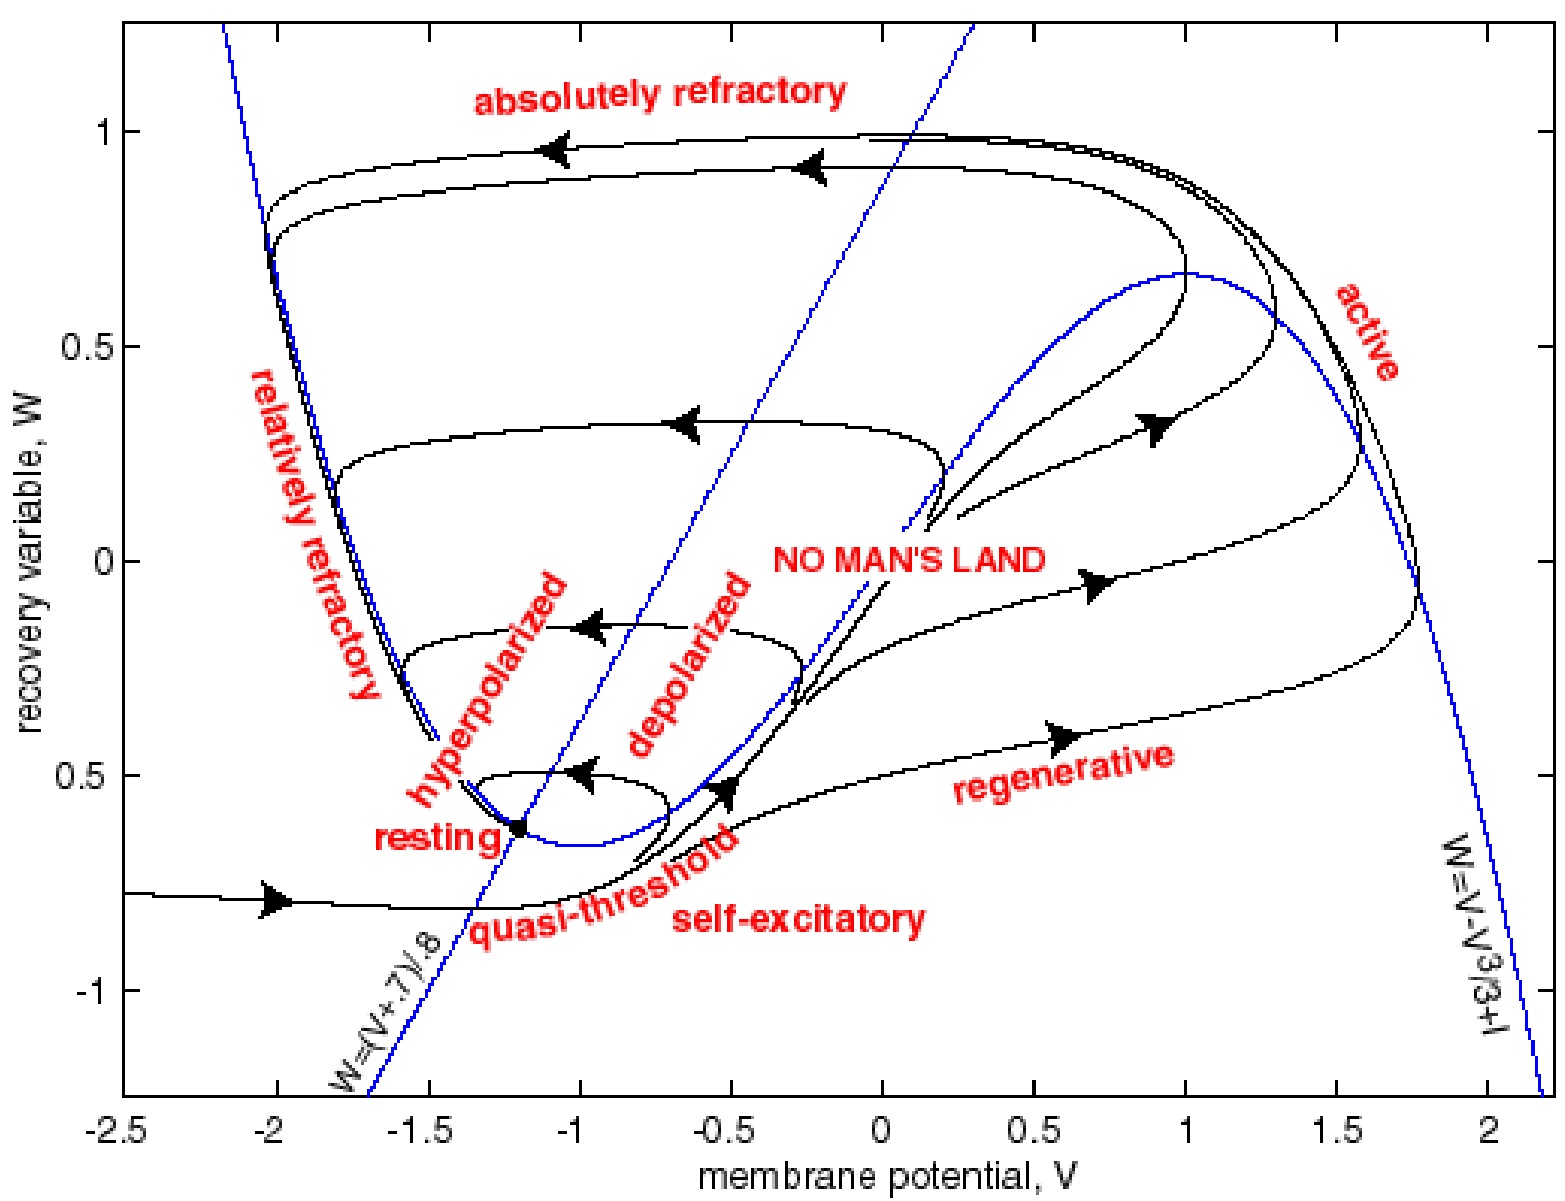
\includegraphics[scale=0.25]{09_6}
    \centering
\end{figure}
It is important to state that the Fitzhugh-Nagumo model is able to explain the \textit{excitation block}
phenomenon, consisting in the cessation of repetitive spiking as the amplitude of the stimulus current
\(I_{app}\) increases. The phases leading to excitation block are the following ones:
\begin{enumerate}
    \item \(I_{app}\simeq{0}\): the equilibrium is on the left branch of the nullcline, thus the
          model is resting.
    \item \(I_{app}\uparrow\): an increasing current shifts the nullcline upward and the equilibrium
          becomes unstable, thus the model is exhibitng a periodic spiking activity.
    \item \(I_{app}\uparrow\uparrow\): a further increase of the stimulus moves the equilibrium to the
          right side of the nullcline and the oscillations are blocked, leaving the neuron in a depolarized state.
\end{enumerate}

\subsection{The Hindmarsh-Rose Model}
This model is used in complex systems, while neuroscientists tend to disregard it, it is 3D, thus employs
three non-linear differential equations. The Hindmarsh-Rose model is aimed at studying the spiking-bursting
behaviour.
\begin{align*}
    \frac{dx}{dt} & =y+\phi{(x)}-z+I_{app}     \\
    \frac{dy}{dt} & =\psi{(x)}-y               \\
    \frac{dz}{dt} & =r\bigl[s(x-x_{R})-z\bigr]
\end{align*}
Note that \(x(t)\) represents the membrane potential, while \(y(t)\) is the rate of fast ion channels
(sodium and potassium), called the spiking variable, and \(z(t)\) is the same for slow ion channels,
denominated the bursting variable.
\begin{figure}[H]
    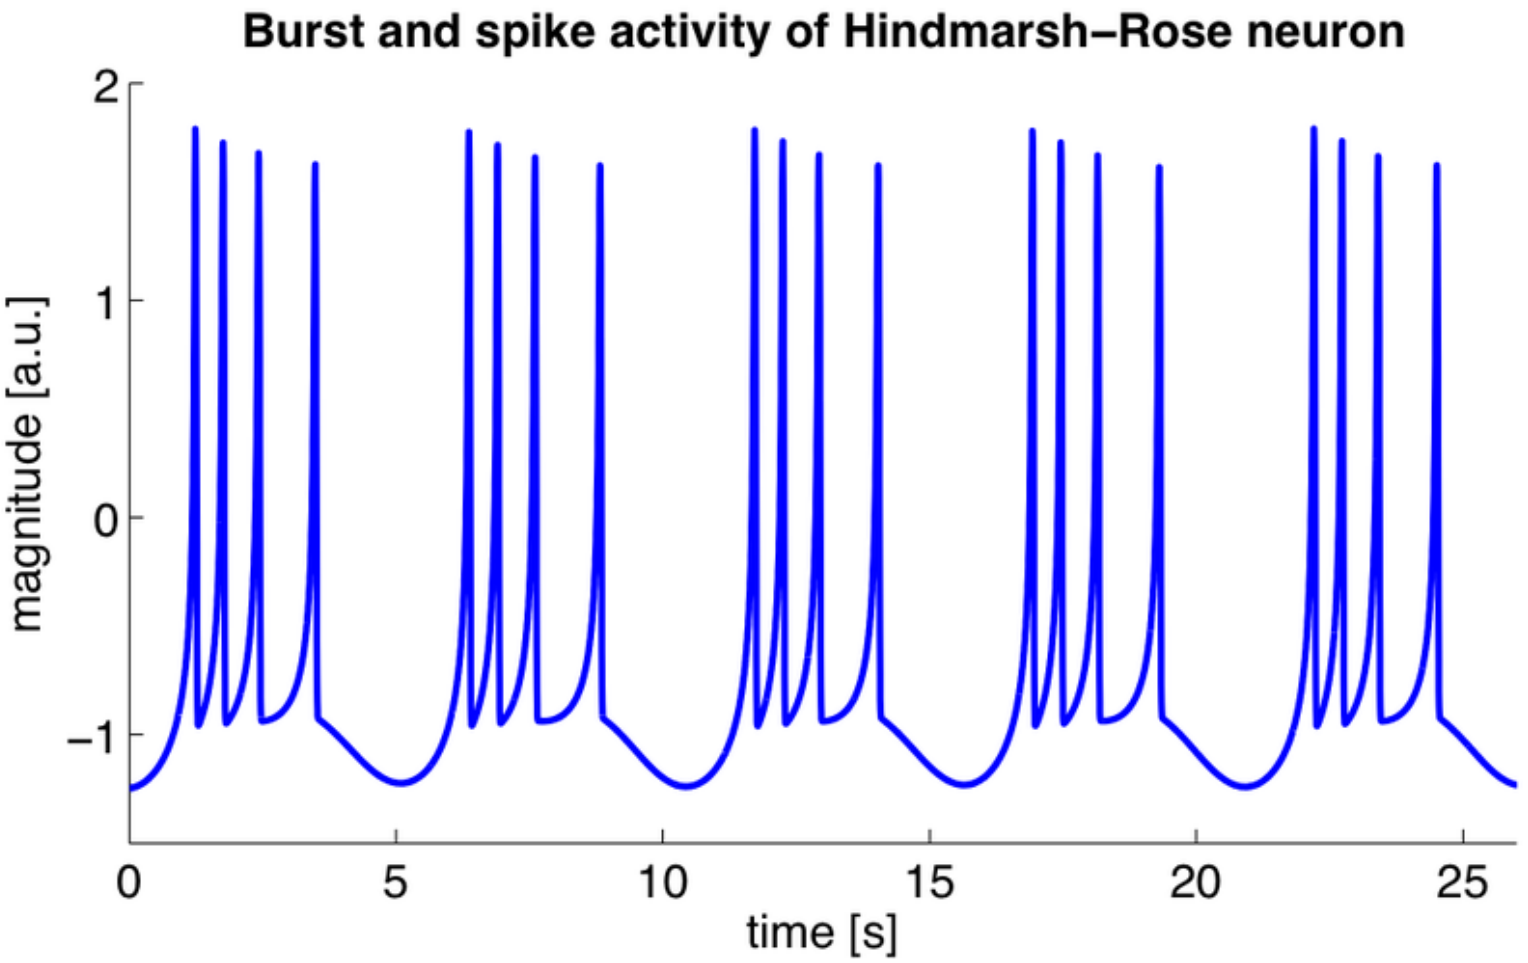
\includegraphics[scale=0.3]{09_7}
    \centering
\end{figure}